\section{Orbit Architecture}
\label{blDOOrb}
In this section the design options in the orbit architecture tree as seen in Figure-\ref{DOOrb1}, Figure-\ref{DOOrb2} and Figure-\ref{DOOrb3} are described. The orbits are divided in four categories: \ac{LEO}, \ac{MEO}, \ac{GEO} and \ac{HEO}. Some orbits like hyperbolic and parabolic trajectories are not included as they are not relevant for the mission.

After the main categories there are subdivisions, which can in turn have subdivisions as well. These subdivisions list the special orbits types that are possible, sometimes there is also a block called ``other''. This is because special orbit types have special constraints, as will be detailed in later sections; whereas the ``other'' block is there to represent all the other possible orbits. It is not possible at this point to determine exact values as the orbit depends on the payload, the power subsystem and the communications subsystem.

All orbits are assumed to be Keplerian orbits, as such the orbit is a plane located in 3D space. Therefore six elements will define the position of the satellite. One example of these elements are the classical orbital elements. The elements are the semimajor axis $a$, the eccentricity $e$, the inclination $i$, the right ascension of the ascending node $\Omega$, the argument of perigee $\omega$ and finally the true anomaly $\nu$. As a reference for the last four terms Figure-\ref{OrbElements} may be used.

\begin{figure} [h]
	\begin{center}
         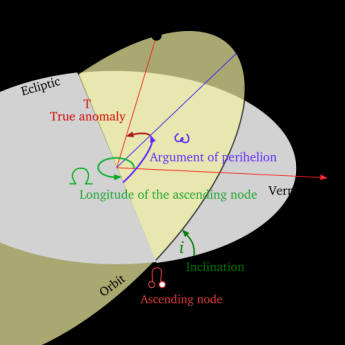
\includegraphics[width=0.75\textwidth,angle=0]{chapters/img/OrbElements.png}
	\caption{Definitions of the inclination $i$, the right ascension of the ascending node $\Omega$, the argument of perigee $\omega$ and the true anomaly $\nu$.}
	\label{OrbElements}
	\end{center}
	\end{figure}
The most important of the four Keplerian elements during this part of the design are the semimajor axis, the eccentricity and the inclination. The remaining elements are not considered until detailed design.

The following sections will each describe one of the four main categories. They are described in the order listed in the first paragraph of this section. However, first the most common orbits are discussed in the following paragraphs.

\subsection {Common orbits}
\label{sec:blOrbCommon}
Some special orbits are repeated multiple times in the orbit architecture trees as shown in Figure-\ref{DOOrb1} to Figure-\ref{DOOrb3}. These common orbits are the polar orbit, the sun synchronous orbit, the sun synchronous polar orbit, the frozen orbit and the repeat orbit.

\begin{enumerate}
	\item Polar orbit:
	This orbit is unique in the sense that the satellite will pass over or closely pass over both poles during a single revolution. As such the angle of incidence $i$ is close to  $\pm$90 [deg]. This setup allows for near global coverage.
	\item Sun synchronous orbit:
	An orbit where the satellite passes over the same ground area at the same local time each revolution. At increasing altitude the inclination increases as well, so above approximately 5000 [km]\cite{larson} this orbit tends to lose its usefulness. 
	\item Sun Synchronous Polar orbit:
	A combination of the previous two items. For this orbit to keep the same local time the altitude should be as low as possible.
	\item Transfer orbit:
	Used to transfer the payload from one orbit to another
	\item Frozen orbit:
	An orbit where there are no long-term changes in argument of perigee and eccentricity. The eccentricity is determined based on a given semimajor axis and inclination.
	\item Repeat orbit:
	An orbit where the satellite comes across the same point on the ground after a integral number of revolutions. A combination of a repeat orbit and a frozen orbit also a possibility.
\end{enumerate}

\subsection{Low Earth Orbit}
\label{sec:blOrb1}
The altitude of a satellite in \acs{LEO} ranges from approximately 80 to 2000 [km]\cite{nasaOrbit}. The lower limit arises from due to the fact of the presence of atmospheric aerodynamic drag, which reduces the velocity and placing it in a different orbit. Placing a satellite in a too low orbit means many attitude corrections have to be made, which is undesirable. The upper limit arises from the inner Van Allen radiation belts, because at 2 to 5 [km]\cite{sse} the radiation is the most intense. Figure-\ref{DOOrb1} shows the design options for the low Earth orbits.

\begin{figure}
\centering
  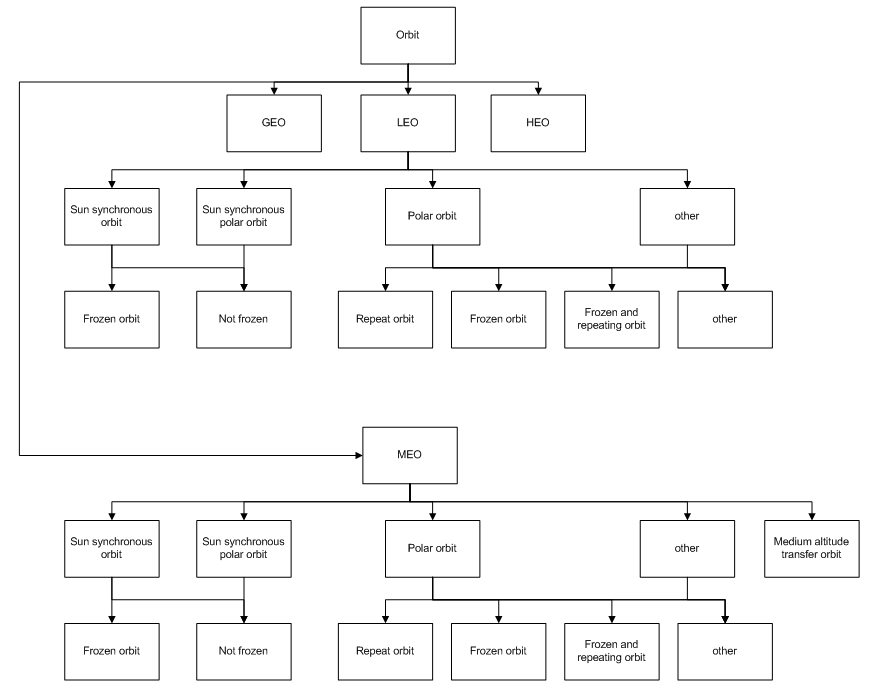
\includegraphics[width=0.75\textwidth,angle=0]{chapters/img/blDOOrb1.jpg}
	\caption{Design option tree for the orbit architecture part 1 of 3.}
	\label{DOOrb1}
\end{figure}

\subsection{Medium Earth Orbit}
\label{sec:blOrb2}
The altitudes for these orbits range from 2000 to 35.700 [km], which is in between the \acs{LEO} and the \ac{GEO}. These are the last orbits where sun synchronous orbits are typically used. This is because of the increase in inclination angle, as mentioned in \ref{sec:blOrbCommon}. Figure-\ref{DOOrb1} shows the design options for the medium Earth orbits.

\subsection{Geosynchronous Orbit}
\label{sec:blOrb3}
Figure-\ref{DOOrb2} shows the design options for the geosynchronous orbits.
This type of orbit is characterized by the satellite completing its orbit in exactly one day. This is not to be confused with a Geostationary orbit, which is a special case of geosynchronous orbit where the eccentricity is 0 and the altitude 35.786 [km].
For the reason mentioned in section \ref{sec:blOrbCommon} sun synchronous orbits are not used at this altitude. \acs{GEO} has two special types of orbits, the supersynchronous and the subsynchronous orbits. 
The apogee of supersynchronous orbits is located located at significantly higher altitude than that of a \acs{GEO} orbit, they are placed under the \acs{GEO} category due relation with the \acs{GEO}. The supersynchronous orbit is also known as a graveyard orbit (or other similar synonyms), as the last name suggests this orbit is used to store dead satellites. Recently another application is used, namely to send the satellite to supersynchronous orbit and change the inclination here and then place the satellite in \acs{GEO}. This is a more efficient maneuver than changing the inclination at \acs{GEO}\cite{jerOrbit}. 
Sometimes a payload is placed in a subsynchronous orbit by the rocket after which the payload has to use its own propulsion to get into \acs{GEO}.

\begin{figure}
\centering
  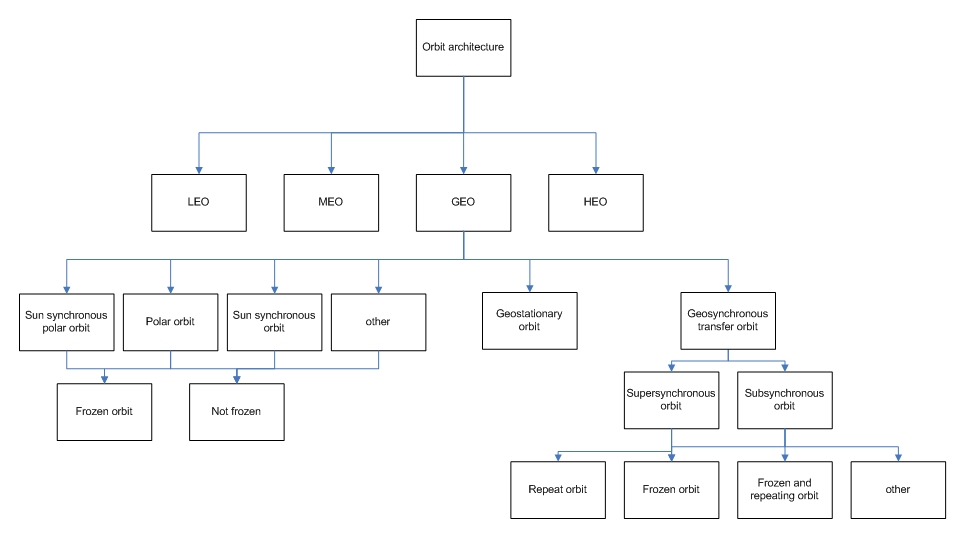
\includegraphics[width=0.75\textwidth,angle=0]{chapters/img/blDOOrb2.jpg}
	\caption{Design option tree for the orbit architecture part 2 of 3.}
	\label{DOOrb2}
\end{figure}

\subsection{High Earth Orbit}
\label{sec:blOrb4}
Continuing the trend indicated in previous sections these orbits are located above the \acs{GEO} orbits. Sun synchronous orbits usually are not used for this orbit as well. 
Figure-\ref{DOOrb3} shows the design options for the high Earth orbit, the \acs{HEllO} discussed in the next part is part of this figure.

\begin{figure}
\centering
  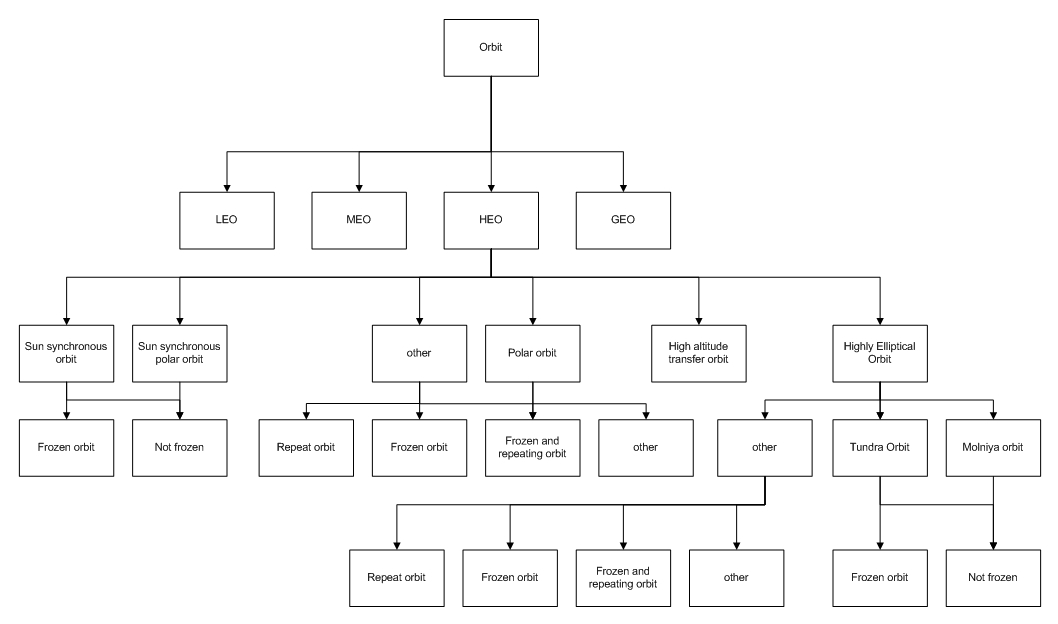
\includegraphics[width=0.75\textwidth,angle=0]{chapters/img/blDOOrb3.jpg}
	\caption{Design option tree for the orbit architecture part 3 of 3.}
	\label{DOOrb3}
\end{figure}

\subsubsection{Highly Elliptical Orbit}
\label{sec:blOrb4.5}
The \ac{HEllO} are defined as a subcategory of the \acs{HEO}, because a satellite in one of these orbits spends most of its time at its apogee. Other than their high eccentricity, the other orbital elements can take any value. Some special orbits are the Molniya orbit and the Tundra orbit. The Molniya orbit has a period of half a sidereal day and the Tundra orbit has a period of a whole sidereal day. For both orbits the inclination often used is 63.4 degrees, this inclination ensures there is no shift or perigee along the orbit. When designing an orbit with a different incidence angle the oblates of the Earth has to be accounted for to negate this effect.